\chapter{BÀI TOÁN LỌC RÁC TIN TỨC CHO HỆ THỐNG PHÁT HIỆN TIN NÓNG}
\ifpdf
    \graphicspath{{Chapter2/Chapter2Figs/PNG/}{Chapter2/Chapter2Figs/PDF/}{Chapter2/Chapter2Figs/}}
\else
    \graphicspath{{Chapter2/Chapter2Figs/EPS/}{Chapter2/Chapter2Figs/}}
\fi

\section{Mở đầu}
Chương này sẽ giới thiệu bài toán lọc rác tin tức cho hệ thống phát hiện tin nóng. Trình bày cơ sở lý thuyết và phát biểu bài toán lọc rác tin tức. Cuối cùng trình bày một số phương pháp tiếp cận bài toán lọc rác tin tức  và các kiến thức liên quan.
\section{Giới thiệu bài toán} %Topic Detection and Tracking}
	\subsection{Các khái niệm cơ bản}
  Để có thể xác định khái niệm rác, ta phải hiểu được khái nhiệm "tin nóng". Le \cite{An:2017} đã định nghĩa khái niệm "tin nóng" như sau:
	\begin{itemize}
    \item \textit{Tin nóng (Hot news)}: những tin viết về một sự kiện mới xảy ra, có tính thời sự, có tầm ảnh hưởng rộng, thu hút được sự chú ý, quan tâm của cộng đồng.
	\end{itemize}

  Ngoài ra Gy\"{o}ngyi và Garcia-Molina định nghĩa "đăng rác" như sau: 
	\begin{itemize}
    \item \textit{Đăng rác (Spamming)}: các hành động có chủ đích của con người nhầm thiên vị tính liên quan của một trang web nào đó, làm sai lệch giá trị của trang web.
	\end{itemize}

  Từ các khái niệm trên ta có định nghĩa "rác" cho bài toán như sau:

  \textbf{Định nghĩa:} Rác là các tin không mang tính chất sự kiện, thời sự, và làm sai lệch kết quả phân tích và xử lý dữ liệu của hệ thống phân loại tin tức. 

  Từ định nghĩa trên ta có thể xác định được các loại tin sẽ được xem là rác:
  \begin{itemize}
    \item \textit{Quảng cáo}: các bài quảng cáo, giới thiệu sản phẩm, các chương trình khuyển mãi, trúng thưởng.
    \item \textit{Tuyển dụng}: các bài đăng tuyển dụng, giới thiệu việc làm của các tổ chức, doanh nghiệp.
    \item \textit{Chia sẻ}: các bài chia sẻ mẹo vặt, thủ thuật, tâm sự, chuyện đời tư, giới thiệu ẩm thực, thời trang, hoặc các kiến thức chung.
  \end{itemize}

	\subsection{Bài toán phân lớp văn bản}
  Bài toán phân lớp văn bản là bài toán có lịch sử lâu đời, một số ghi nhận cho thấy nó bắt đầu từ những năm 1800s, tuy nhiên tới nay vẫn chưa có một sự thống nhất nào về phương pháp tốt nhất cho bài toán phân lớp \cite{zechner:history}. 
  
	Theo Zechner \cite{zechner:history}, bài toán phân lớp văn bản gồm các thành phần chính cần quan tâm: 
		\begin{itemize}
			\item Loại phân lớp: supervised hoặc unsupervised.
			\item Mục tiêu: đối tượng thành phần của văn bản mà ta muốn quan tâm.
			\item Kho từ vựng: kích thước và chất lượng của kho từ vựng ảnh hưởng lớn đến việc phân lớp.
			\item Features: đặc trưng của văn bản dùng cho việc phân lớp.
			\item Bộ phân lớp: thuật toán máy học dùng cho việc phân lớp.
		\end{itemize}

	\subsection{Bài toán lọc rác tin tức}
  Bài toán lọc rác hay còn được biết đến như là bài toán phát hiện rác (Spam detection) là một dạng bài toán phân lớp văn bản nhị phân. Tức là chỉ có hai lớp: "rác" và "không rác". Đối với hệ thống phát hiện tin nóng cũng như các hệ thống phân tích và xữ lý dữ liệu khác, việc phát hiện và lọc rác phải được diễn ra trước khi quá trình phân tích và xử lý dữ liệu bắt đầu để đảm bảo quá trình phân tích và xử lý dữ liệu chính xác và đáng tin cậy.

  Mặc dù nguồn dữ liệu mà chúng ta quan tâm là tin tức từ các trang báo điện tử chính thống, số lượng nguồn tin, chủ đề tin và số lượng tin rất lớn dẫn đến việc chất lượng dữ liệu tin tức không được đảm bảo cũng như tính chất dữ liệu không được phù hợp với nhu cầu của hệ thống. Do đó việc lọc rác tin tức là cần thiết cho việc khai thác và sử dụng nguồn dữ liệu tin tức một các hiệu quả.

  \subsection{Phát biếu bài toán lọc rác tin tức cho hệ thống phát hiện tin nóng}
  Cho trước một bài báo $d_i$i. Mục tiêu của bài toán là tìm ra được nhãn $l_i$ của bài báo $d_i$ và nhãn đó nhận một trong hai giá trị: "rác" và "không rác".
	
\section{Các nghiên cứu liên quan}
Vấn đề phát hiện và lọc rác là một vấn đề lâu đời và kinh điển đối với bài toán phân lớp văn bản. Do đó số lượng nghiên cứu xoay quan vấn đề này cũng rất lớn và đa dạng. Phần lớn các nghiên cứu cho đến ngày nay tập trung vào việc phát hiện rác cho email, web và mạng xã hội. 

Sahami và cộng sự \cite{Sahami1998ABA} sử dụng các tiếp cận Bayesian vào vấn đề lọc rác cho email. Thực nghiệm cho thấy các bộ phân lớp đạt được hiệu suất cao hơn khi ta cân nhắc các tính năng đặc trưng theo domain và nội dung văn bản của email. Ngày nay thì các phương pháp phát hiện và lọc rác cho email đã khá hoàn thiện, và các phương pháp phát hiện và lọc rác Bayesian được áp dụng rộng rãi trong các email client và server.

Rothwell và cộng sự\cite{rothwell2004intelligent} đã xây dựng một hệ thống phát hiện các thông điệp rác bằng cách sử dụng neural network. Khi một thông điệp được đưa vào hệ thống nó sẽ được phân rã và các thông số thống kê trong thông điệp đó sẽ được thu thập bở bộ phân tích số liệu. Một neural network được huấn luyện bằng cách sử dụng sự kết hợp tuyến tính linh hoạt đề thay đổi các trọng số cùng với bộ phân tích số liệu thống kê sẽ được dùng để quyết định xem một thông điệp có phải là rác hay không.  

Idris và cộng sự\cite{IDRIS201533} đã xây dựng một hệ thống phát hiện rác cho email sử dụng thuật toán negative selection và particle swarm optimization (NSA-PSO). Hệ thống áp dụng thuật toán local outlier factor (LOF) để tính toán độ mở rộng của không gian không rác để thu thập được các tính năng tốt nhất cho việc phân lớp. Mô hình NSA-SPO được dùng để phân biệt giữa rác và không rác trong các mạng client-server.

Vấn đề phát hiện rác cho web thì khó khăn hơn vì độ lớn và tốc độ thay đổi nhanh chóng. Gy\"{o}ngyi và cộng sự \cite{Gyongyi:2004:CWS:1316689.1316740} đề xuất sử dụng thuật toán TrustRank để đo kiểm điểm tin cậy của đồ thị Web. Dựa trên điểm tin cậy, các trang web tốt sẽ được đánh giá cao hơn va những trang web xấu có thể được search engine bỏ qua. 

Benczúr và cộng sự\cite{benczur} tiếp cận bài toán phát hiện web rác bằng các xác định các trang web được back linked bởi nhiều trang khác, bằng việc tính toán điểm SpamRank để đánh giá lại PageRank thật sự xứng đáng của một trang web. 

Phát hiện rác trên các nền tảng mạng xã hội cũng là một trong các chủ đề nóng trong lĩnh vực này. Jin và cộng sự\cite{jin} đã đề xuất một hệ thống phát tự động thu hoạch các hoạt động đăng tin rác trên ác trang mạng xã hội bằng cách sử dụng các bộ định vị xã hội đối với các cơ sở người dùng lớn. Hệ thống dùng các đặc trưng của cả hình ảnh và văn bản để xác định các nội dung rác, và sử dụng thuật toán gom cụm GAD cho dữ liệu quy mô lớn.

Wang cũng xây dựng một hệ thống phát hiện rác cho dữ liệu Twitter sử dụng thuật toán phân lớp Naive Bayes. Hệ thống thức hiện phân lớp dựa trên các đặc tính mạng xã hội của Twitter và đặc tính nội dung của dữ liệu văn bản. Theo kết quả đo kiểm đánh giá thì độ chính xác của hệ thống đạt đến 89\%\cite{5741690}

\section{Giới thiệu một số phương phát trừu tượng hóa dữ liệu văn bản} \label{distances}
Do máy tính không thể đọc hiểu và xử lý được dữ liệu thuần văn bản, ta cần có một phương pháp trừu tượng hóa dữ liệu văn bản thành các con số mà máy tính có thể hiểu được.
\subsection*{Term Frequency - Inverse Document Frequency (TF-IDF)}
Trong lĩnh vực thu thập thông tin, TF-IDF là một dữ liệu số dùng để thể hiện độ quan trọng của một từ trong một một tập hợp hoạc một kho từ vựng \cite{rajaraman_ullman_2011}. Nó thường được dùng trong việc thu thập thông tin, text mining và user modeling. Giá trị của TF-IDF tăng theo tỉ lệ với số lần một từ xuất hiện trong một văn bản, nhưng thường bị giảm lại theo tần xuất của từ đó trong toàn kho từ vựng, vì một từ có thể chỉ đơn giản là nó phổ biến hơn các từ khác. Ngày nay, TF-IDF là một trong những phương pháp tính trọng số cho các từ phổ biến nhất; 83\% các hệ thống khuyến nghị dựa trên văn bản trong lĩnh vực thư viện điện tử sử dụng TF-IDF \cite{Beel2016}.

TF-IDF gồm có hai thành phần chính Term Frequency (TF) và Inverse Document Frequency (IDF).

TF của từ $t$ trong văn bản $d$ được thể hiện dưới dạng $tf(t,d)$. Ta có nhiều cách tính TF, trong đó cách đơn giản nhất là đếm số lần một từ xuất hiện trong một văn bản. Nếu ta gọi số lần từ $t$ xuất hiện trong văn bản $d$ là $f_{t,d}$ thì ta có $tf(t,d) = f_{t,d}$

IDF là thước đo lượng thông tin một từ cung cấp, có nghĩa là liệu từ đó hiếm gặp hay xuất hiện xuyên suốt trong kho từ vựng. IDF được tính bằng công thức:
\begin{equation}
  idf(t, D) = \log\frac{N}{1 + \abs{\{d \in D: t \in d\}}}
\end{equation}

Trong đó:
\begin{itemize}
  \item $D$: kho từ vựng.
  \item $N$: số lượng văn bản trong kho từ vựng.
  \item $\abs{\{d \in D: t \in d \}}$: số lượng văn bản và có xuất hiện từ $t$. 
\end{itemize}
	\subsection*{Word Vector}
Word vector là một hình thức biểu diễn các từ trong một kho từ vựng dưới dạng các vector. Các từ thường xuất hiện cùng nhau trong các nhiều ngữ cảnh khác nhau thì sẽ được biểu diễn bằng các vector gần với nhau trong không gian vector \cite{mikolov:word2vec}. Tập hợp các kỹ thuật để nhận vào input là một kho từ vựng và cho ra một không gian vector tương ứng được gọi là word2vec.

  Word vector thường được sử dụng trong các công cụ tìm kiếm và dịch thuật do nó cung cấp thông tin về sự tương qua ngữ nghĩa giữa các từ và các ngữ cảnh cũng như giữa các từ với nhau.

\section{Các phương pháp tiếp cận phổ biến}
Phân lớp là quá trình xác định xem một đối tượng sẽ thuộc về lớp nào dựa trên việc quan sát các đối tượng khác mà lớp của chúng đã được xác định từ trước. Thông thường, các đối tượng cần phân lớp sẽ được phân tích thành các thuộc tính có thể đo đếm được. Một thuật toán dùng để phân lớp, hay còn được gọi là một bộ phân lớp, sẽ dựa trên các thuộc tính đó để ánh xạ các đối tượng input mới vào lớp của chúng. Đây là một trong những tác vụ chính của lĩnh vực khai thác dữ liệu.

Bài toán phân lớp bao gồm nhiều thuật toán khác nhau, trong phạm vi của khóa luận chúng ta sẽ chỉ quan tâm đến các thuật toán: Support vector machine, Naive Bayes, và J48 decision tree.
\subsection{Thuật toán phân lớp Support Vector Machine (SVM)}
\subsubsection{Giới thiệu}
Support vector machine hay còn gọi là support vector network là một thuật toán phân lớp dành cho các bài toán phân lớp nhịphân. SVM thực hiện phân lớp bằng việc ánh xạ các vector lên một không gian nhiều chiều. Trên không gian này sẽ sinh ra một mặt phẳng quyết định tuyến tính phân tách hai lớp dữ liệu \cite{Cortes1995}.
	\begin{figure}[ht]
    \centering
			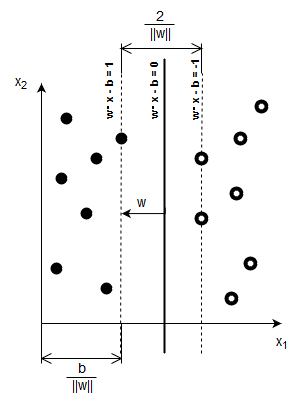
\includegraphics[width=0.65\textwidth]{linearSVM.png}
      \caption{\textit{Minh họa về một bộ phân lớp SVM tuyến tính. Siêu phẳng với lề cực đại và các margin của một bộ SVM được học từ các mẫu được gán nhãn thành hai lớp. Những mẫu nằm trên margin được gọi là support vector}}
	\end{figure}
\subsubsection{Ưu điểm, hạn chế}
		Ưu điểm:
		\begin{itemize}
			\item Rất hiệu quả khi tập dữ liệu có chiều không gian lớn.
			\item Vẫn hiệu quá trong các trường hợp số chiều lớn hơn số lượng dữ liệu.
      \item Chỉ sử dụng một phần dữ liệu huấn luyện để ra quyết định (các dữ liệu huấn luyện này là các support vector).
      \item Có nhiều kernel để sử dụng cho chức năng ra quyết định, thể hiện sự đa dạng, phân lớp dữ liệu tốt.
		\end{itemize}
		Nhược điểm:
		\begin{itemize}
			\item Nếu như số chiều lớn hơn nhiều so với số lượng dữ liệu thì cho hiệu năng thấp.
			\item Vì thuật toán SVM là thuật toán phi xác suất nên không cung cấp các ước lượng xác suất trực tiếp để kiểm tra độ chính xác mà dùng phương pháp trung gian là k-fold cross validation để kiểm tra với chi phí cao.
		\end{itemize}
\subsubsection{SVM với bài toán lọc rác tin tức}
Bài toán lọc rác văn bản là một bài toán phân lớp nhị vân với các vector đặc trưng có số chiều rất lớn nên đây là một bài toán rất phù hợp cho việc sử dụng thuật toán SVM. 
%========================================================================================================================
\section{Thuật toán Naive Bayes} 
\subsection{Giới thiệu}
Thuật toán Naive Bayes là một thuật toán phân lớp xác suất đơn giản dùng để tính một tập các xác suất bằng cách đếm tần suất và kết hợp của các giá trị trong một tập cho trước. Thuật toán sử dụng định luật Bayes sẽ giả định rằng tất cả các chiều(attributes) của dữ liệu là độc lập với nhau. Các giả định rằng các chiều là độc lập với nhau rất khó để có thể xuất hiện trong thực tế. Tuy nhiên giả thiết ngây ngô này lại mang lại những kết quả phân lớp tốt cho nhiều bài toán phân lớp \cite{dimitoglou2012comparison}.

Định lý Bayes cho phép tính xác suất xảy ra của một sự kiện ngẫu nhiên A khi biết sự kiện liên quan B đã xảy ra. Xác suất này được ký hiệu là P(A|B), và đọc là “xác suất của A nếu có B”. Đại lượng này được gọi xác suất có điều kiện hay xác suất hậu nghiệm vì nó được rút ra từ giá trị được cho của B hoặc phụ thuộc vào giá trị đó. Theo định lí Bayes, xác suất xảy ra A khi biết B sẽ phụ thuộc vào 3 yếu tố: Xác suất xảy ra A của riêng nó, không quan tâm đến B. Kí hiệu là P(A) và đọc là xác suất của A. Đây được gọi là xác suất biên duyên hay xác suất tiên nghiệm, nó là “tiên nghiệm” theo nghĩa rằng nó không quan tâm đến bất kỳ thông tin nào về B. Xác suất xảy ra B của riêng nó, không quan tâm đến A. Kí hiệu là P(B) và đọc là “xác suất của B”. Đại lượng này còn gọi là hằng số chuẩn hóa (normalising constant), vì nó luôn giống nhau, không phụ thuộc vào sự kiện A đang muốn biết. Xác suất xảy ra B khi biết A xảy ra. Kí hiệu là P(B|A) và đọc là “xác suất của B nếu có A”. Đại lượng này gọi là khả năng (likelihood) xảy ra B khi biết A đã xảy ra. Chú ý không nhầm lẫn giữa khả năng xảy ra B khi biết A và xác suất xảy ra A khi biết B. Tóm lại định lý Bayes sẽ giúp ta tính ra xác suất xảy ra của một giả thuyết bằng cách thu thập các bằng chứng nhất quán hoặc không nhất quán với một giả thuyết nào đó. Khi các bằng chứng tích lũy, mức độ tin tưởng vào một giả thuyết thay đổi. Khi có đủ bằng chứng, mức độ tin tưởng này thường trở nên rất cao hoặc rất thấp, tức là xác xuất sảy ra giả thuyết sẽ thay đổi thì các bằng chứng liên quan đến nó thay đổi.	
\subsection{Ưu điểm, hạn chế}
Ưu điểm:
\begin{itemize}
  \item Đơn giản, nhanh, dễ cài đặt
  \item Nếu điều kiện giả định độc lập của thuật toán Naive Bayes là đúng, thì nó sẽ hội tụ nhanh hơn nhiều khi so sánh với các mô hình phân biệt như là logistic regression.
  \item Ngay cả khi điều kiên giả định độc lập của thuật toán Naive Bayes không được đảm bảo một cách tuyệt đối, thì thuật toán này vẫn hoạt động một cách ổn định và đáng tin cậy trong thực tế. 
  \item Không cần nhiều dữ liệu huấn luyện.
  \item Khả năng mở rộng cao. Thuật toán này có thể mở rộng một cách tuyến tính theo số lượng các predictor và các điểm dữ liệu.
  \item Có thể dùng cho các bài toán phân lớp nhị phân lẫn các bài toán phân lớp đa lớp.
  \item Có thể thực hiện các dự đoán có tính xác suất.
  \item Xử lý được cả dữ liệu rời rạc lẫn dữ liệu liên tục.
  \item Không có các đặc tính thừa thải.
\end{itemize}
Nhược điểm:
\begin{itemize}
  \item Trên thực tế điều kiện giả định độc lập là gần như không thể xảy ra, điều này dẫn đến sự hao hụt về độ chính xác.
\end{itemize}
\subsection{Thuật toán Naive Bayes và bài toán lọc rác tin tức}
Naive Bayes là một trong các thuật toán được dùng rất phổ biến trong việc phát hiện và lọc rác cho email. Nó là một trong những kỹ thuật cơ bản và lâu đời nhất trong lĩnh vực này. Do đó, đề tài nãy cũng sẽ tìm hiểu và áp dụng Naive Bayes vào bài toán lọc rác tin tức.

\section{Thuật toán J48}
\subsection{Giới thiệu}
Thuật toán J48(C4.5) là một thuật toán sử dụng cây quyết định (decision tree) cho việc phân lớp. Thuật toán sẽ tạo ra môn cây nhị phân. Bằng cách sử dụng cây quyết định, cách tiếp cận này cũng thường đước sử dụng trong bài toán phân lớp. Cây quyết định sẽ được xây dựng để mô hình hóa quá trình phân lớp.

Cây quyết định (Decision Tree) là một cây phân cấp có cấu trúc được dùng để phân lớp các đối tượng dựa vào dãy các luật (series of rules). Các thuộc tính của đối tượng (ngoại trừ thuộc tính phân lớp – Category attribute) có thể thuộc các kiểu dữ liệu khác nhau (Binary, Nominal, ordinal, quantitative values) trong khi đó thuộc tính phân lớp phải có kiểu dữ liệu là Binary hoặc Ordinal. Tóm lại, cho dữ liệu về các đối tượng gồm các thuộc tính cùng với lớp (classes) của nó, cây quyết định sẽ sinh ra các luật để dự đoán lớp của các đối tượng chưa biết (unseen data).
\begin{figure}[H]
\centering
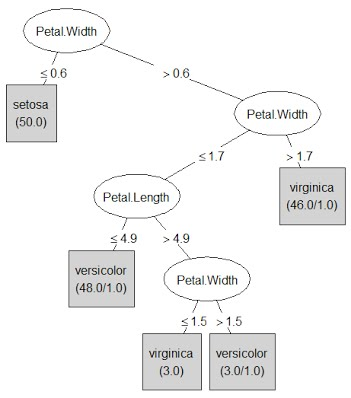
\includegraphics[width=0.9\linewidth]{Chapter2/Chapter2Figs/J48.png}
\caption{Ví dụ về cây quyết định. Thực hiện phân lớp các loài hoa: setosa, versicolor, virginica; dựa trên độ dài và độ rộng của cánh hoa}
\end{figure}
\subsection{Ưu điểm, hạn chế}
Ưu điểm:
\begin{itemize}
  \item Có khả năng chọn ra các đặc tính có tính phân biệt sâu sắc nhất.
  \item Phân loại được dữ liệu mà không cần thực hiện quá nhiều thao tác tính toán.
  \item Xử lý tốt dữ liệu nhiễu và không hoàn chỉnh.
\end{itemize}
Nhược điểm:
\begin{itemize}
  \item Tỉ lệ lỗi phân lớp cao khi tập dữ liệu huấn luyện có kích thước nhỏ so với số lượng lớp.
  \item Tốc độ huấn luyện tăng nhanh chóng khi kích thước tập dữ liệu và số lượng các đặc tính tăng.
\end{itemize}
\section{Các độ đo đánh giá các thuật toán phân lớp}
\subsection{Precision và Recall}
Trong lĩnh vực nhận diện mẫu, thu thập thông tin và phân lớp nhị phân, precision là tỉ lệ giữa số lượng các đối tượng cần quan tâm đối với tổng các số lượng trả về, trong khi đó recall là tỉ lệ số lượng các đối tượng cần quan tâm trả về đối với tổng số các đối tượng cần quan tâm.

Đối với các tác vụ phân lớp, precision của một lớp dữ liệu là số lượng các đối tượng true positive (TP) (số đối tượng được phân lớp đúng vào lớp positive) chia cho tổng số đối tượng được phân lớp là positive (tổng của cả true positive và positive - các đối tượng phân lớp sai là positive). Trong ngữ cảnh này, recall được xác định bằng tổng số đối tượng true positive chia cho tổng số đối tượng thuộc về lớp positive. Giá trị precision tuyệt đối 1.0 của lớp C có nghĩa là tất cả các đối tượng được phân vào lớp C đúng là thuộc về lớp C (nhưng không nói gì về số lượng các đối tượng thuộc về lớp C bị phân sai vào các lớp khác), trong khi đó, giá trị recall tuyệt đối 1.0 có nghĩa là tất các đối tượng thuộc lớp C đều được phân vào lớp C (nhưng không nói gì về số lượng các dối tượng thuộc về các lớp khác cũng được phân sai vào lớp C).

Trong các tác vụ phân lớp, ta sử dụng các khái niệm \textit{true positve (TP), false positive (FP), true negative (TN), false negative (FN)} để so sánh kết quả phân lớp. Các từ \textit{positive} và \textit{negative} dùng để thể hiện kết quả dự đoán của bộ phân lớp (hay còn gọi là \textit{expectation}). Các từ \textit{true} và \textit{false} được dùng để chỉ kết quả đánh giá của chúng ta từ bên ngoài về kết quả phân lớp (hay còn gọi là  \textit{observation}).

Khi đó, precision và recall được xác định bằng:
\begin{center}
  $Precision = \frac{TP}{TP + FP}$
\end{center}
\begin{center}
  $Recall  = \frac{TP}{TP + FN}$
\end{center}
\subsection{F-Measure}
F-measure là một phương thức kết hợp giá trị của precision và recall bằng cách lấy giá trị trung bình điều hòa (harmonic mean) của chúng:
\begin{center}
  $F = 2\times \frac{precision\times recall}{precision\times recall}$
\end{center}
Giá trị của F-measure thể hiện mức độ cân bằng của hai giá trị precision và recall, và gần bằng giá trị trung bình của chúng khi chúng xấp xỉ nhau.
\subsection{Receiver operating characteristic (ROC) area}
Trong  xác suất, đường cong ROC là một dạng đồ thị thể hiện khả năng phân tích của một bộ phân lớp nhị phân khi có đa dạng ngưỡng phân biệt.

Đường cong ROC được tạo ra bằng việc bằng cách vẽ biểu đồ dựa trên tỉ lệ true positive (recall) và true negative (specifity). Và diện tich nằm dưới đường cong ROC (ROC area) bằng với xác suất một bộ phân lớp sẽ đánh giá một đối tượng positive được chọn ngẫu nhiên cao hơn một đối tượng negative được chọn ngẫu nhiên (ngầm đình là postive xếp hạng cao hơn negative)\cite{Fawcett:2006:IRA:1159473.1159475}.

\section{Kết chương}
Chương này đã đề cập đến các nghiên cứu liên quan đến bài toán lọc rác tin tức, các thuật toán được sử dụng trong đề tài, và các phương pháp để đánh giá các thuật toán đó.